\documentclass[11.5pt]{article}
\usepackage[table]{xcolor}
\definecolor{lightgray}{gray}{0.9}
\usepackage{multirow} 
\usepackage{lscape}
\usepackage{filecontents}
\usepackage[left=2.5cm,top=2.5cm,right=2.5cm,bottom=2.5cm]{geometry}
\usepackage{amsmath}
\usepackage{array}
\usepackage{caption}
\usepackage{longtable}
\usepackage{placeins}
\usepackage{graphicx}
\usepackage{subcaption}
\usepackage{setspace}
%\usepackage[active,tightpage]{preview}
\usepackage{natbib}
\bibpunct{(}{)}{,}{a}{}{;} 
\usepackage{url}
\usepackage{nth}
\usepackage{authblk}
\usepackage{listings}
% for the d in integrals
\newcommand{\dd}{\; \mathrm{d}}
\newcommand{\tc}{\quad\quad\text{,}}
\newcommand{\tp}{\quad\quad\text{.}}
\bibliographystyle{apalike}



\begin{document}


\section*{Figures}

\begin{figure}[h!]
\centering
\caption{Temporary life expectancy for states (black line), record life
expectancy (red) and low mortality benchmark by sex, 1990-2010.}
\label{Fig1:temp}
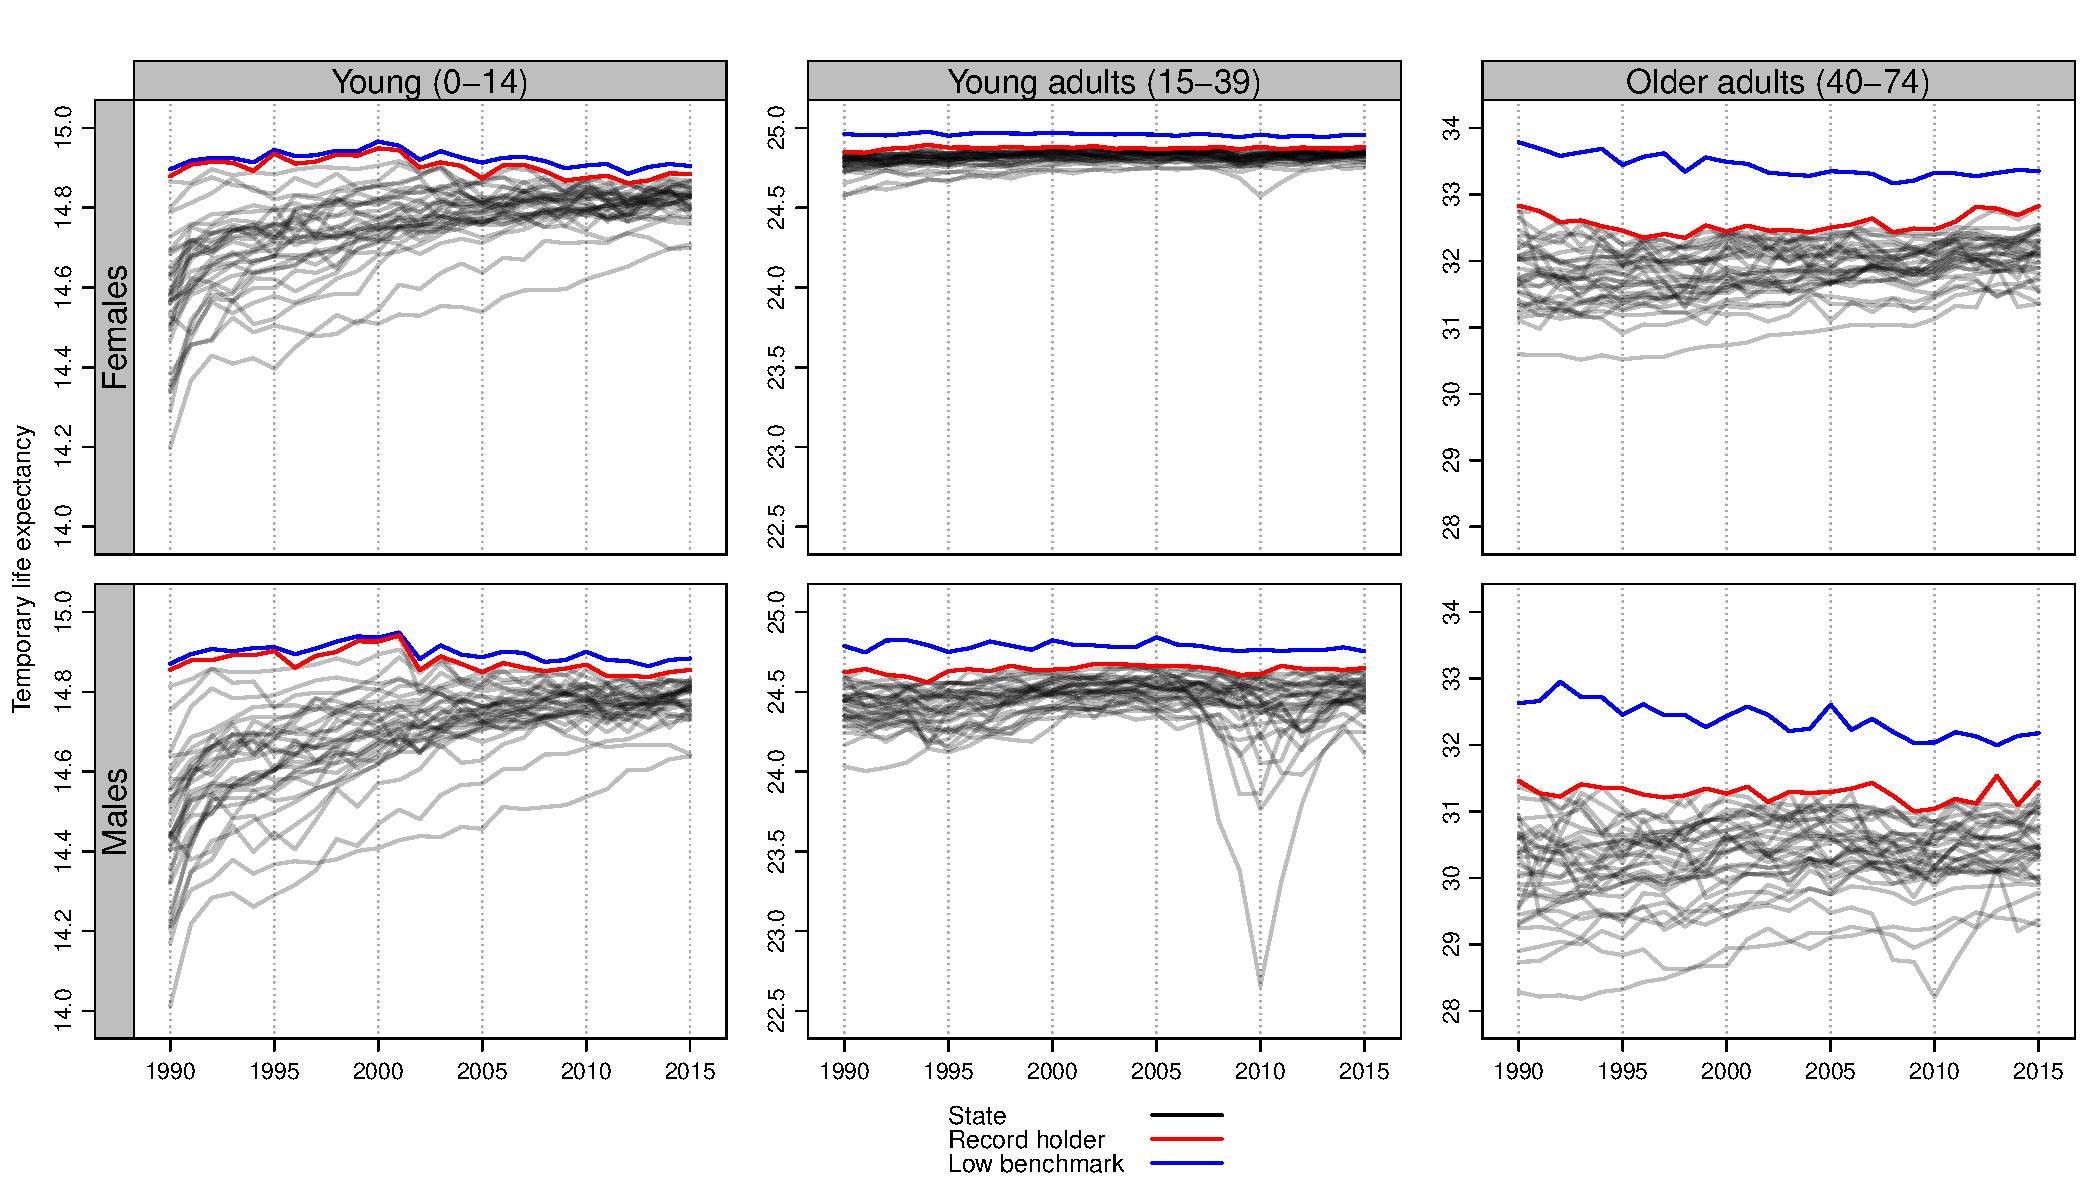
\includegraphics[scale=.5]{Figure_1.pdf}

Note: Y-axis are not in the same scale in order to capture major trends over the period. Source: calculations based on INEGI and SOMEDE files. 
\end{figure}



\begin{figure}[h!]
\centering
\caption{Survival inequality (coefficient of variation) by age group and sex, 1990-2010.}
\label{fig:Gini}
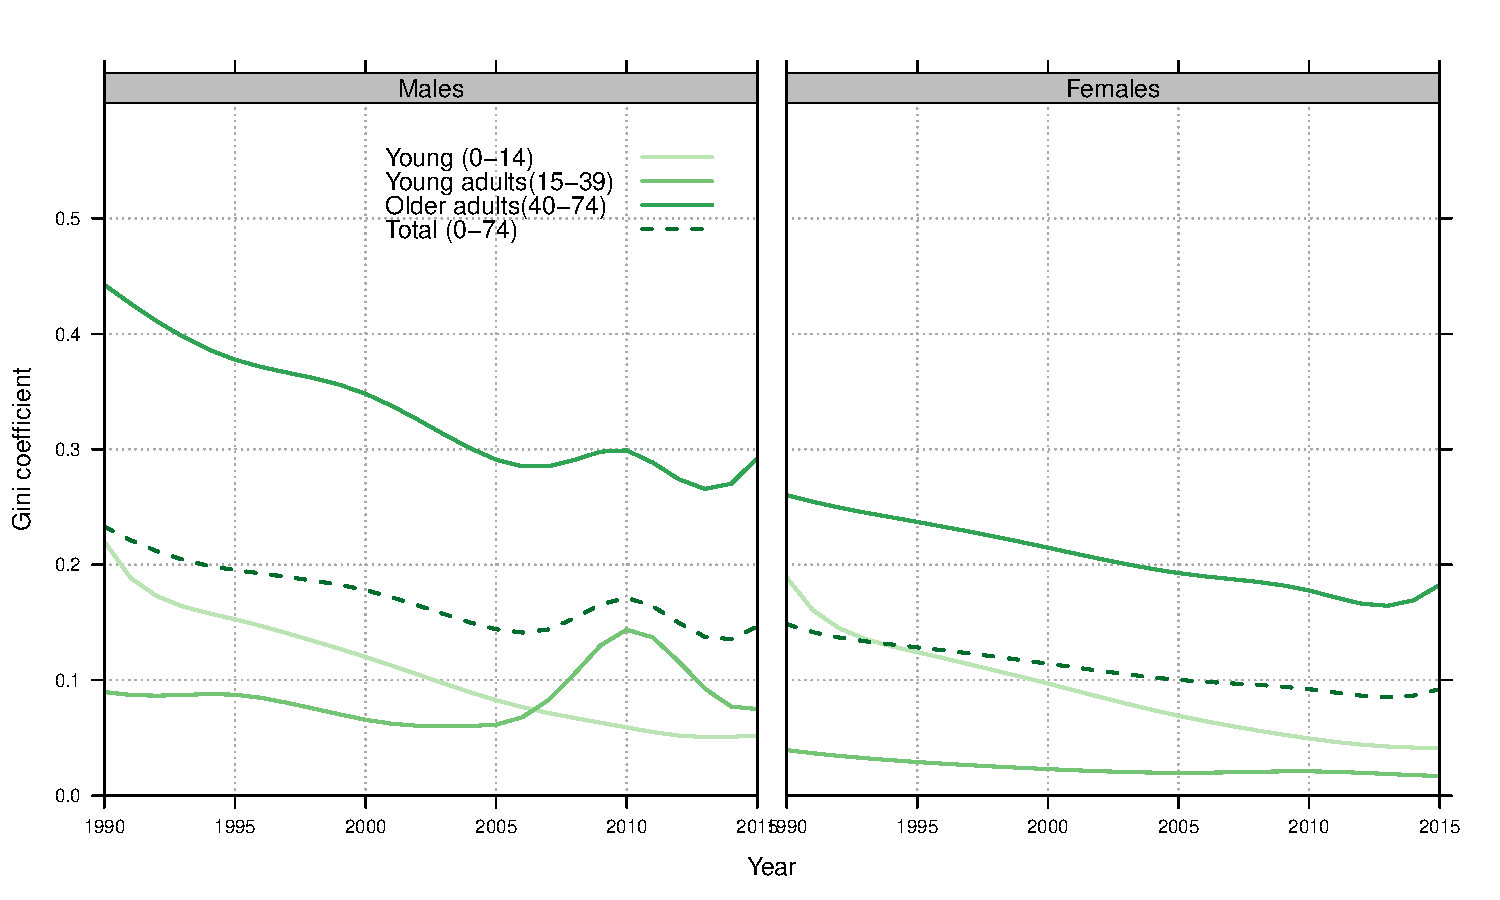
\includegraphics[scale=.5]{Gini_fig.pdf}

 Source: calculations based on INEGI and SOMEDE files.
\end{figure}



\begin{figure}[h!]
\centering
\caption{Cause-specific contributions to state differences from low mortality benchmark for older male adults, 1990-2010.}
\label{fig:e40_74_males}
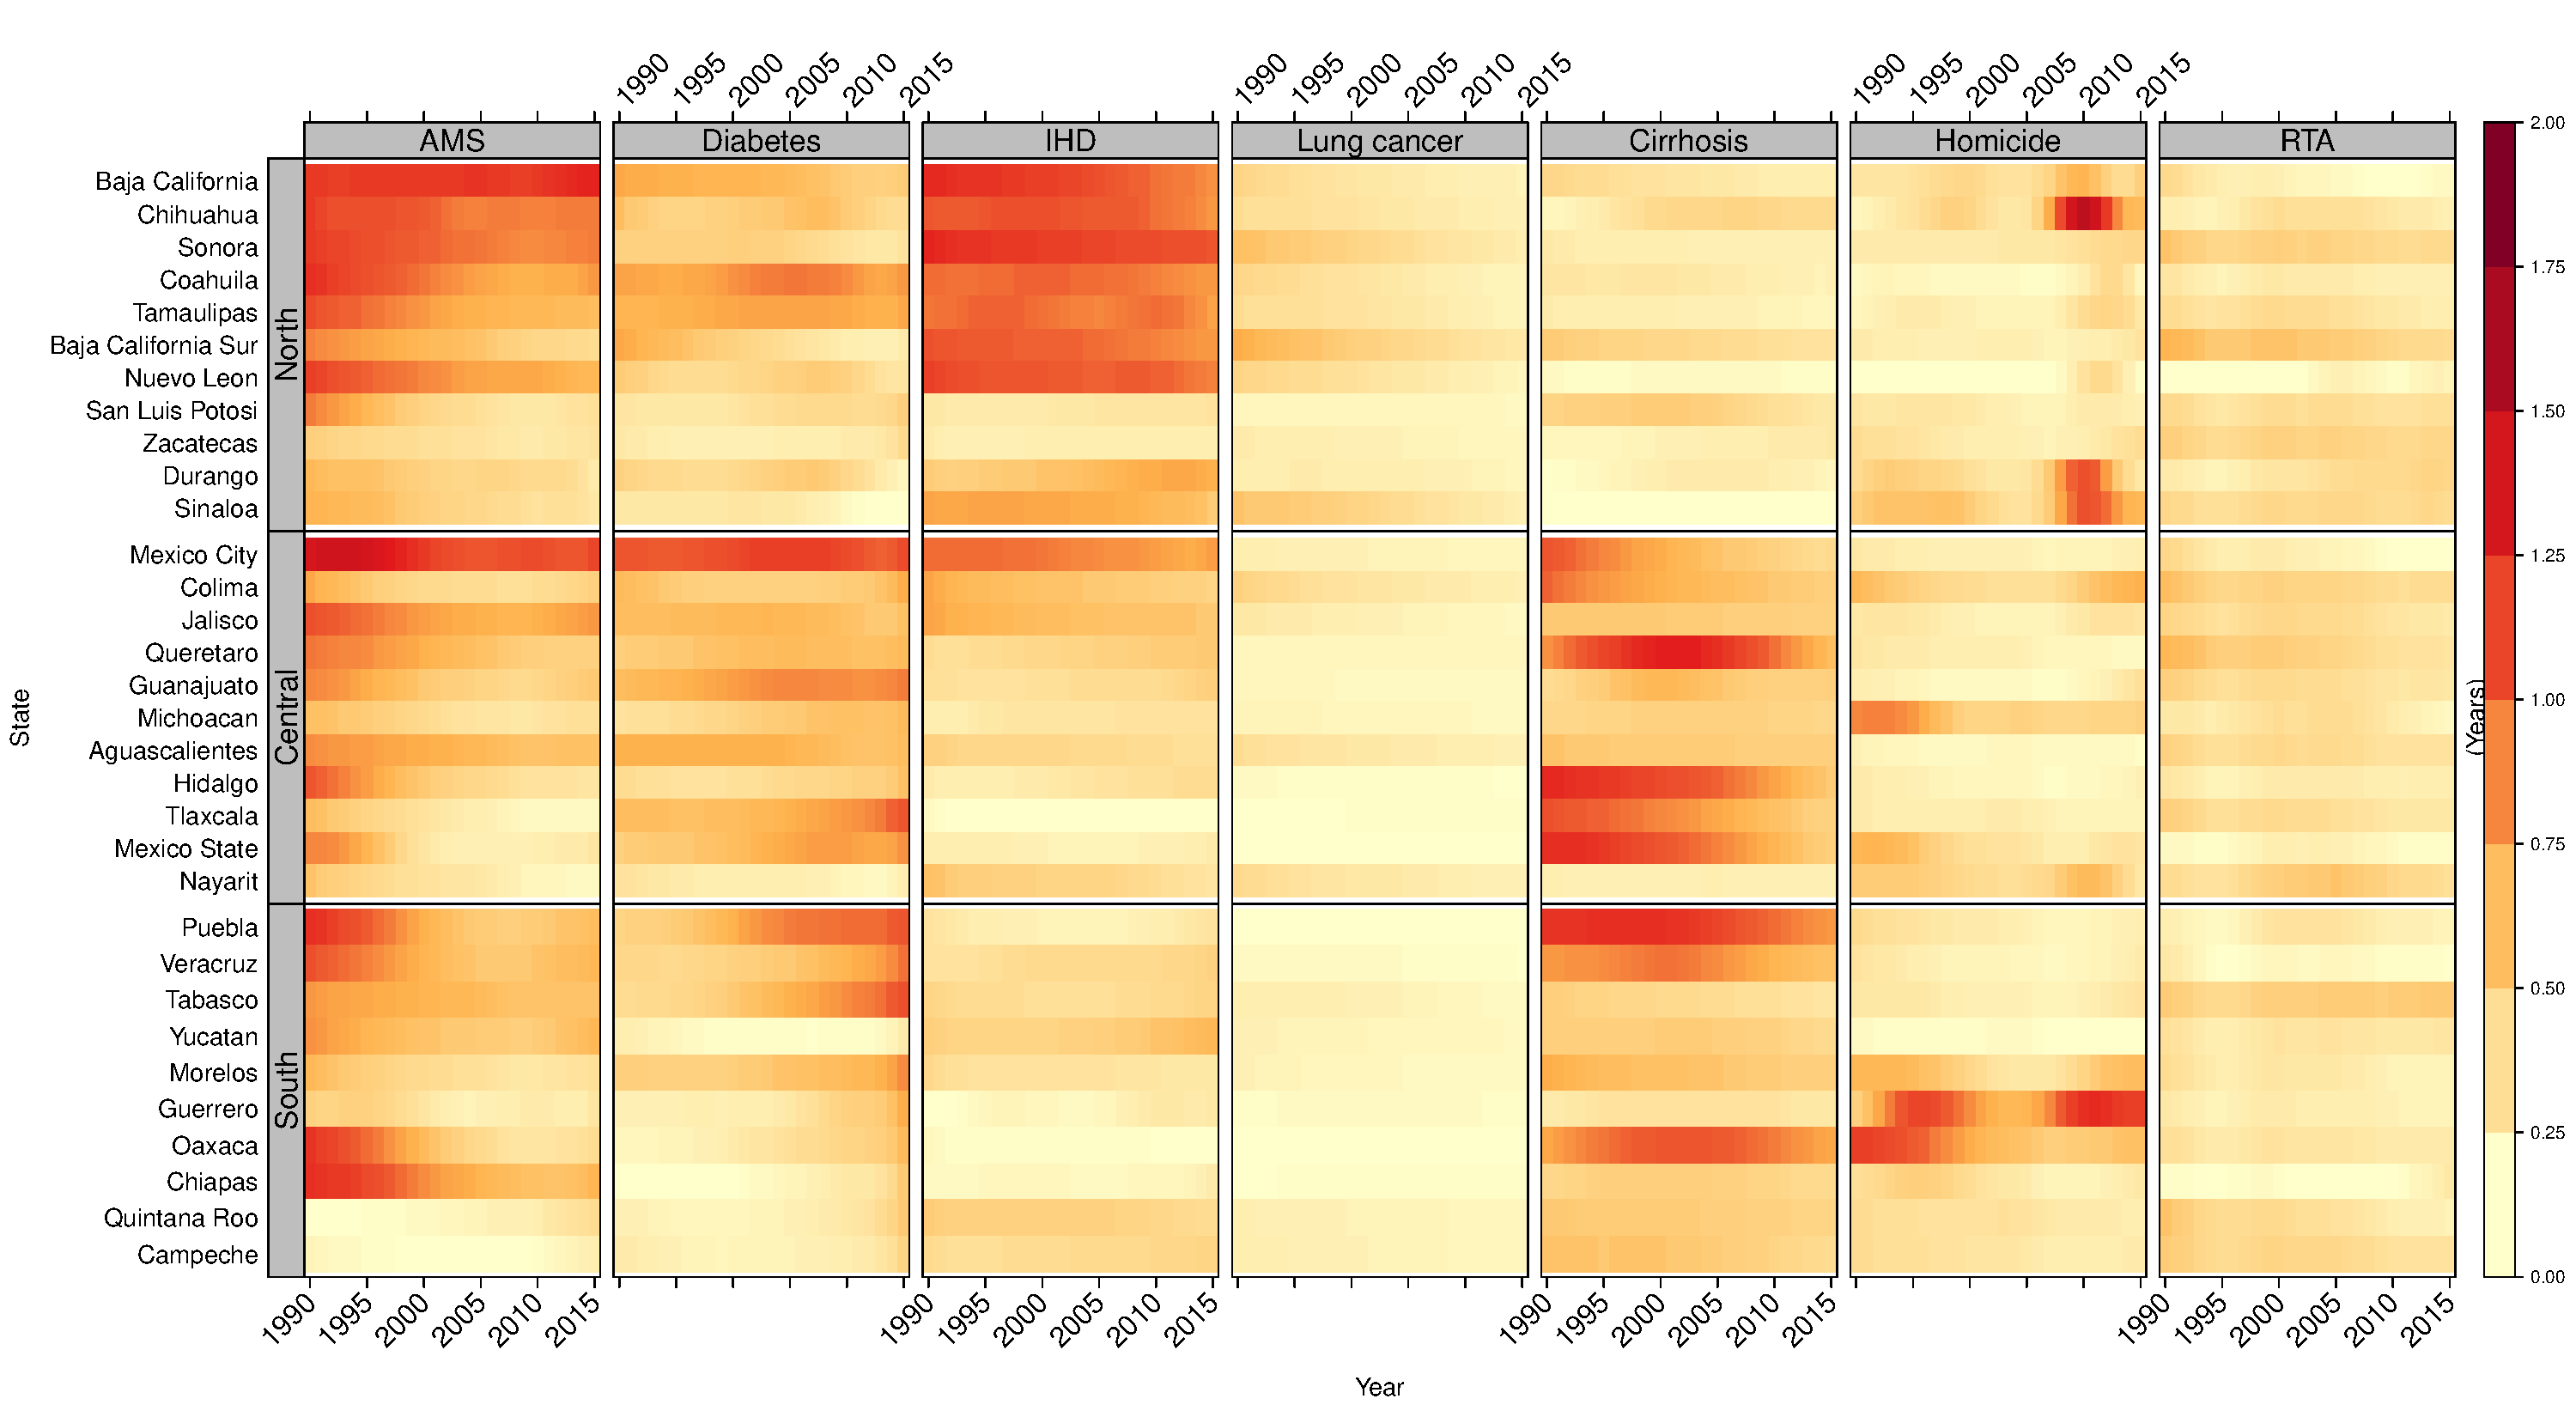
\includegraphics[scale=.31]{Adult_Male_heatmap.pdf}
Note: AMS, is the acronym for amenable to medical service, IHD for isquemic heart diseases and RTA stands for road traffic accidents. Source: own calculations based on INEGI and SOMEDE files. 
\end{figure}

\end{document}